
\documentclass[a4paper,12pt]{article}
\usepackage[utf8]{inputenc}
\usepackage{graphicx}
\usepackage[magyar]{babel}
\usepackage{t1enc}

\begin{document}

\author{Elek István}

\title{Catalog  \linebreak  \linebreak \small Felhasználói leírás \linebreak \linebreak}


\date{\today}


\setcounter{tocdepth}{3}
%\frontmatter
\maketitle
\newpage
\tableofcontents
\newpage
%\mainmatter

\section{Catalog}

A \textbf{Catalog} alrendszer nagy tömegben keletkező képek (csak \textit{jpg} és \textit{tif} formátumú képek) rendszerezésére, adatbázisba szervezésére való (ehhez sqlite-ot használ a program). Az adatok és a képek gyors szemrevételezését is lehetővé teszi. A \textbf{DataStock} alrendszer használata enélkül is lehetséges, hiszen bármely képet használatba vehetjük vele. A \textbf{Catalog}ot olyankor célszerű használni, amikor több száz vagy több ezer képet kívánunk egységesen kezelni, a leíró adataik alapján keresést végezni.

\subsection{Első lépések}

\begin{itemize}
	\item Másoljuk be egy könyvtárba a catalog.zip fájlt.
	\item Bontsuk ki.
	\item Ahová kibontottuk, onnan indítható a catalog.exe, nem kell külön telepíteni.
	\item Az első induláskor még nincs képi adatbázis, ezért panaszkodni fog a hiányára (\ref{fig:missingdb}. ábra):
	
	\begin{figure}[h]
		\centering
		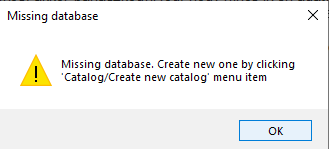
\includegraphics[width=8cm]{missingdb.png}
		\caption{A 'Missing database' üzenet}
		\label{fig:missingdb}
	\end{figure}
	
	\item Ezután megjelenik a program fő formja, ahol kreálhatunk egy új, üres adatfájl (\ref{fig:createnewcatalog}. ábra) (a default név 'dronimagecatalog.s3db', de lehet bármi más is)
	
	\begin{figure}
		\centering
		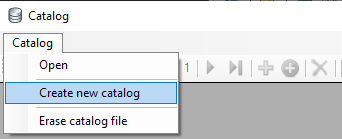
\includegraphics[width=8cm]{createnewcatalog.png}
		\caption{A \textit{Create new catalog} menü}
		\label{fig:createnewcatalog}
	\end{figure}

	\item Ezután a 'Open' menüre klikkelve megnyílik az üres adatbázis-fájl.
	
	\item Ha már van létező adatbázis (pl. dronimagecatalog néven), akkor megjelenik a tartalma egy táblázatban a program fő formján (\ref{fig:catalog0}. ábra). Ritka eset, de ha nincs, akkor panaszkodni fog, hogy nincs ilyen adatbázis  –- mert például kitörültük a fájlrendszerből, de a catalog még úgy emlékszik, hogy van ilyen fájl. Kattintsunk az OK-ra, majd nyomjuk meg az F2 gombot -– bal felső sarok környéke a billentyűzeten. Ekkor megjelenik egy 'Catalog' nevű menü. Válasszuk ki a 'Create new catalog' almenüt, amely létrehoz egy 'dronimagecatalog' nevű adatbázist, és benne egy üres adattáblát, amelynek 'images' lesz a neve. Ide fognak képződni a felvett képek adatai.
	
	\begin{figure}
		\centering
		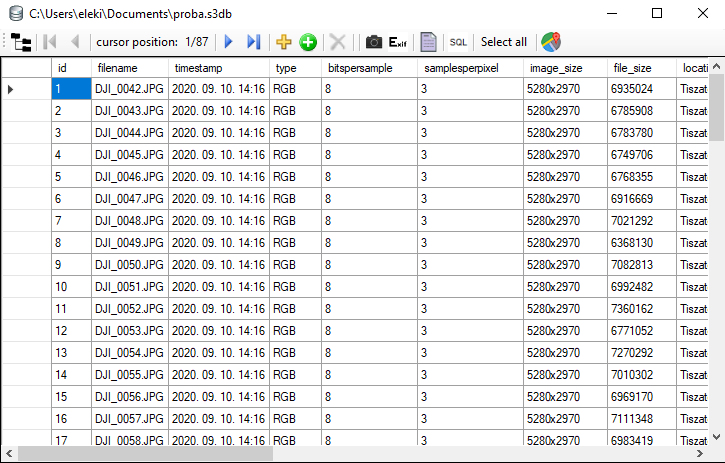
\includegraphics[width=13cm]{catalog0.png}
		\caption{A \textit{Catalog} fő formja}
		\label{fig:catalog0}
	\end{figure}

	\item Normál indulásnál a menürendszer nem látszik (F2-t megnyomva jelenik meg és tűnik el)
	
	\item Az ikonok elmondják, hogy mit tudnak, ha az egeret föléjük mozgatjuk.
	
\end{itemize}

\subsection{A fájlrendszer előkészítése}

\begin{itemize}
	\item Kreáljunk egy könyvtárat 'DRON\_IMAGES' néven valahol a fájlrendszerben.
	
	\item Klikkeljünk az 'open folder tree' ikonra (
\includegraphics{open_folder_structure.png}). Ekkor megnyílik a 'Folder structure' nevű ablak (\ref{fig:folder_struc}. ábra).
	
	\item Klikkeljünk a 'Set destination folder' nevű menü gombra, majd keressük meg és válasszuk ki a 'DRON\_IMAGES' nevű könyvtárat. Ezzel megadtuk a kép katalógus helyét a fájlrendszerben, amire ezentúl emlékezni fog a program, ha újra megnyitjuk a 'Folder structure' ablakot. 
	
	\item Keressük meg a flash driven-on (ami a dronon a képeket tárolja) azt a könyvtárat, ahol az éppen most készített képek vannak. Ha a jobb oldali ablakban megjelennek a fájlok, klikkeljünk a 'Save files to '\verb|c:\DRON_IMAGES| folder' ikonra (
\includegraphics{save.png}). Ennek hatására az egész könyvtár tartalma átmásolódik a flash driveról a 'DRON\_IMAGES' nevű könyvtárba.
	
	\item Ennek hatására a 'DRON\_IMAGES' nevű könyvtárban megjelenik egy új directory, aminek a neve az első fájl mentésének időpontja. Ez a könyvtár fogja tartalmazni az adott időben történt repülés képeit.
\end{itemize}

\begin{figure}
	\centering
	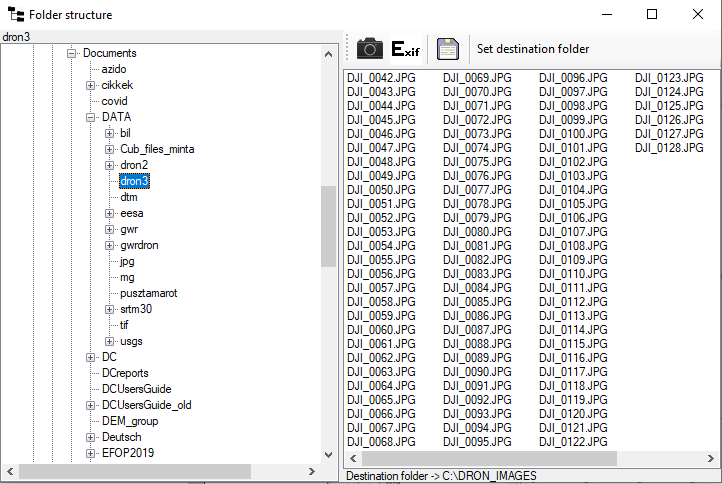
\includegraphics[width=13cm]{folder_struc.png}
	\caption{A \textit{Folder structure} ablak}
	\label{fig:folder_struc}
\end{figure}

\subsection{Az adatbázis feltöltése}

\begin{itemize}
	\item Kétféleképpen tölthetjük fel az adatbázist: vagy egyenként (vagy multiselecttel több fájlt is) vagy egy directory-t kijelölve tömegesen, annak teljes tartalmát (csak jpg és tif fájl, más nem). A fájlonkénti kijelöléshez klikkeljünk a sárga plusz jelre (
\includegraphics[width=0.5cm]{plus.png}), a teljes directory kijelöléséhez a zöld karikában fehér kereszt ikonra (
\includegraphics[width=0.5cm]{addfolder.png}).
	
	\item Bármelyikre klikkeltünk, felbukkan a 'Editable image attributes' nevű ablak (\ref{fig:editableimageattribute}. ábra), ahol megadhatjuk azokat az adatokat, amelyek minden most beemelendő képre vonatkoznak. A többi adatot a program automatikus feltölti (fájlnév, long, lat, timestamp, folder, stb.).
	
	\begin{figure}
		\centering
		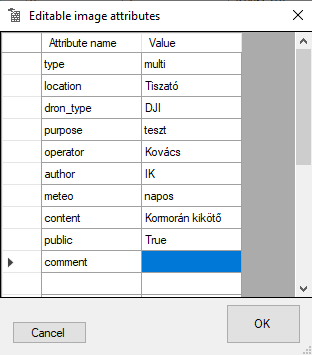
\includegraphics[width=6cm]{editableimageattributes.png}
		\caption{Az \textit{Editable image attributes} ablak}
		\label{fig:editableimageattribute}
	\end{figure}
	
	\item A táblázat nem automatikus adatai szerkeszthetők, amik el is mentődnek, amint a következő rekordra lépünk.
	
	\item A fényképezőgép ikonra 
\includegraphics[width = 0.5 cm]{camera.png}) kattintva megjelenik az aktuális rekordhoz tartózó kép. Az 'Exif' (
\includegraphics[width = 0.6 cm]{exif.png}) feliratú ikon az aktuális rekordhoz tartozó kép exif adatait mutatja meg egy külön ablakban.
\end{itemize}

\subsection{Funkciók}

Az adatokat mutató táblázat felett egy ikonosztáz látható, amelyen a főbb funkciók lettek elhelyezve. A 
\includegraphics[width = 0.5 cm]{filesystem.png} ikon megnyit egy a fájlrendszert nézegető ablakot, hol megnézhetjük az adatok forrását, mint pl. egy pendrive-ot, ami közvetlenül a drón adattároló eszköze, és amelyen a legfrissebb mérési adatok vannak(\ref{fig:folder_struc}. ábra). A kiválasztott fájlokat (az egész könyvtárat) a \textit{DRON\_IMAGES} nevű könyvtárba másolja be. Amúgy ezt az első használat során meg kell adni (\textit{Set destination folder}). A másolást a 
\includegraphics[width=0.5cm]{save.png} ikonra való klikkelés végzi.

Az adatbázisban már bent lévő képeket a 
\includegraphics[width = 0.5 cm]{camera.png}  ikonnal, míg a hozzá tartozó EXIF adatokat az 
\includegraphics[width = 0.5 cm]{exif.png}  ikonnal nézhetjük meg.

Új képeket, egyenként a 
\includegraphics[width=0.5cm]{plus.png} ikonnal, míg tömegesen, vagyis egy egész directory tartalmát, a 
\includegraphics[width=0.5cm]{addfolder.png} ikonnal adhatjuk hozzá az adatbázishoz. A hozzáadás egyben az adatbázis feltöltését is elvégzi, persze csak azokat az adatokat, amelyek a képekből kinyerhetők. Interaktívan is hozzáadhatók adatok, ha azokat a megfelelő mezőbe beírjuk. A 
\includegraphics[width=0.5cm]{del.png} ikonnal egy kijelölt rekordot törölhetünk. Nemcsak a leíró adatok törlődnek (az 'images' nevű tábla kijelölt rekordja), hanem a \textit{DRON\_IMAGES} könyvtárból is a kijelölt kép fájl (UNDO nincs!).

\begin{figure}
	\centering
	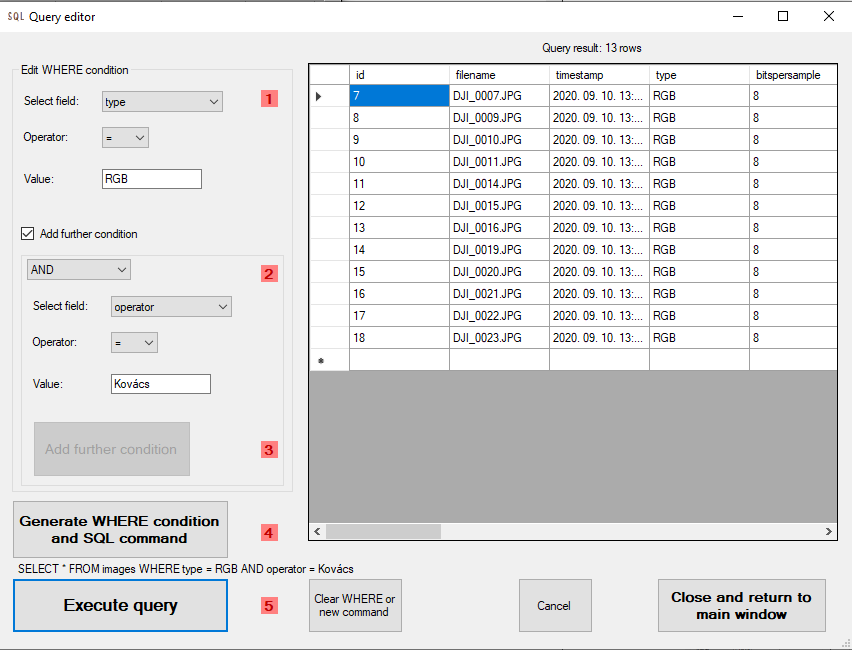
\includegraphics[width=12cm]{sqleditor.png}
	\caption{Az \textit{Sql editor} ablak}
	\label{fig:sqleditor}
\end{figure}

Az 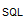
\includegraphics[width=0.5cm]{sql.png} ikonnal SQL parancsokat állíthatunk össze, amelyekkel tetszőleges feltétel szerint kereshetünk (legyűjthetünk) a rendelkezésre álló képek paraméterei alapján. Az \ref{fig:sqleditor}. ábrán olyan képek legyűjtésének eredménye látható, amelyek a Tiszán készültek, és a kép típusa 'multispektrális'. Az 'Sql editor' az Sql-t nem, vagy csak alapszinten ismerők számára is használható. 
(Az Sql-ben járatos felhasználók számára előhívható egy rejtett Sql parancssor, amely azért rejtett, mert hozzá nem értők kezében veszélyes fegyver lehet, amellyel súlyos károkat is lehet okozni az adatbázisban. Akik biztosak az Sql tudásukban, azok az F12 gomb megnyomásával előhívhatják az Sql parancssort, amely eltüntethető, ha újra megnyomjuk az F12 gombot. Nemcsak lekérdező, hanem non query típusú parancsok is kiadhatók. A parancs \textbf{Enter}rel hajtható végre.)


A 
\includegraphics[width = 0.5 cm]{sheet.png} ikonnal egy adott mérésre vonatkozó riport fájlt nézetünk meg, vagy hozhatunk létre, amelybe olyan adatokat tehetünk bele, amelyeket a mérési körülmények miatt, vagy bármilyen szempontból érdekesnek találunk, de nem az egyes képekhez kötöttek.

\subsection{Lekérdezés}

\begin{itemize}
	\item  Az 'SQL' feliratú ikonra klikkelve (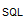
\includegraphics[width=0.5cm]{sql.png}) megjelenik egy 'Query editor' nevű ablak. Itt ki lehet választani, hogy melyik mezőre kérdezünk, milyen feltételt szabunk.
	
	\item pl. select field: type;  Operator: =; Value: RGB $\rightarrow$ 
	WHERE type=RGB. Ha itt vége, akkor click to 'Generate WHERE condition and Sql command' majd 'Execute query'. 
	
	\item Ha új lekérdezés lesz, akkor előtte click to 'Clear WHERE or new command'. Vigyázat, az Sql editor case sensitive (rgb !=  RGB)
	
	\item Összetettebb lekérdezésekhez az előbbihez hasonló lekérdezés után klikkeljünk az 'Add further condition' nevű check boxra. 
	
	\item Ha kész vagyunk egy further feltétellel, klikkeljünk az 'Add further condition'- gombra. Ha az utolsót is hozzáadtuk, akkor klikkeljünk a 'Generate WHERE condition and Sql command' majd az 'Execute query'-re. Ha jó volt az sql parancs, akkor megjelenik az eredmény az adatrácsban.
	
	\item Ha meg vagyunk elégedve az eredménnyel, klikkeljünk a 'Close and return to main window' gombra. Ekkor becsukódik a 'Query editor' ablak, és a lekérdezés eredménye megjelenik a fő ablakban. Itt nézegethetjük a képek listáját.
	
	\item A 'Select all' feliratú gombra a bal egérgombbal klikkelve az összes képet legyűjthetjük az adatbázisból, amelyek adatai meg is jelennek az adatrácsban.
	
	\item A 'Select all' feliratú gombra a jobb egérgombbal klikkelve az összes képet kijelölhetjük az  adatrácsban (\ref{fig:mapviewer_select_all}. ábra). Ezt olyankor hasznos, amikor térképen akarjuk megjeleníteni a legyűjtött képek centroidjait. Ehhez még rá kell kattintani a 
\includegraphics[width = 0.5 cm]{mapviewer_ikon.png} ikonra. Ekkor megjelennek a 'Map viewer' ablakban (\ref{fig:mapviewer}. ábra felső része) a képek centroidjai. Ha úgy klikkeltünk a 
\includegraphics[width = 0.5 cm]{mapviewer_ikon.png} ikonra, hogy nem jelöltünk ki egyetlen képet sem, akkor az ELTE Térképtudományi és Geoinformatikai Intézet helye jelenik meg a térképen (a \ref{fig:mapviewer}. ábra alsó része).
	
		\begin{figure}
		\centering
		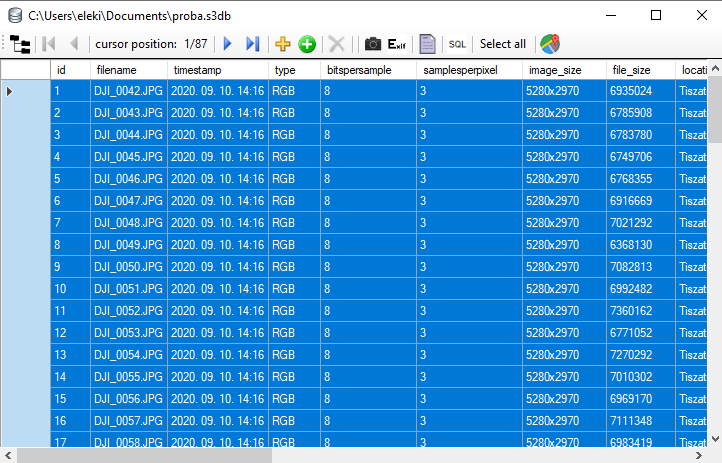
\includegraphics[width=12cm]{mapviewer_select_all.png}
		\caption{A \textit{Map viewer} ablak}
		\label{fig:mapviewer_select_all}
	\end{figure}
	
	\begin{figure}
		\centering
		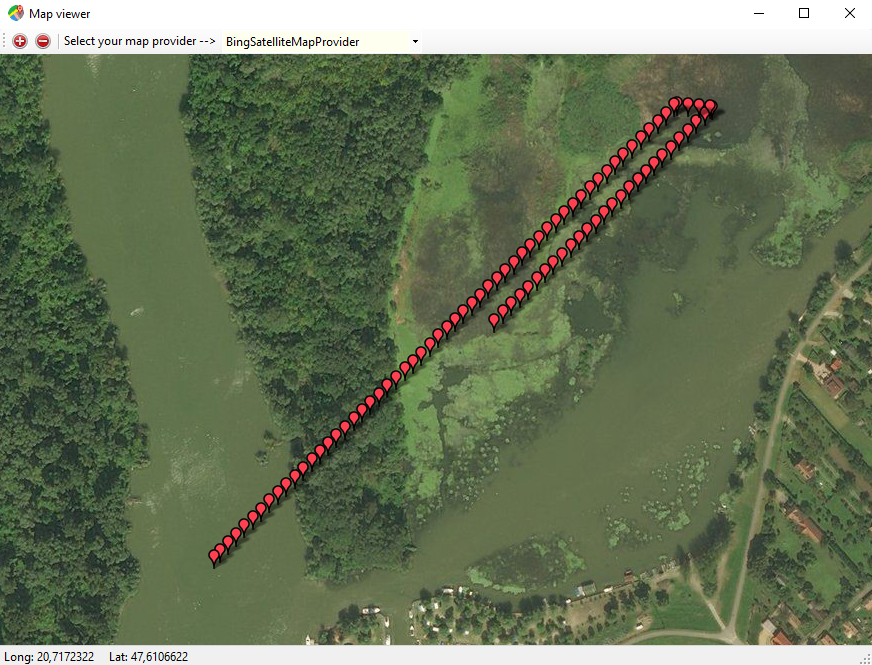
\includegraphics[width=12cm]{mapviewer.png}
	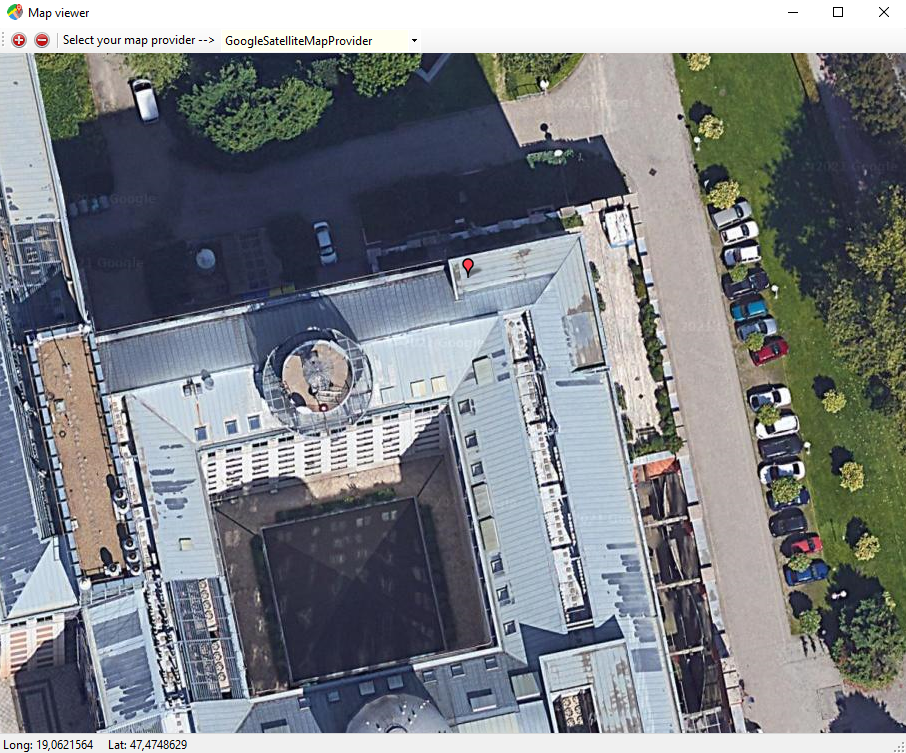
\includegraphics[width=12cm]{tegeta.png}		
		\caption{A \textit{Map viewer} ablak. Felső részen a Kormorán kikötő (Tiszafüred), míg az alsón az ELTE látható}
		\label{fig:mapviewer}
	\end{figure}	
	
\end{itemize}

\end{document}